\documentclass[]{article}
\usepackage{lmodern}
\usepackage{amssymb,amsmath}
\usepackage{ifxetex,ifluatex}
\usepackage{fixltx2e} % provides \textsubscript
\ifnum 0\ifxetex 1\fi\ifluatex 1\fi=0 % if pdftex
  \usepackage[T1]{fontenc}
  \usepackage[utf8]{inputenc}
\else % if luatex or xelatex
  \ifxetex
    \usepackage{mathspec}
  \else
    \usepackage{fontspec}
  \fi
  \defaultfontfeatures{Ligatures=TeX,Scale=MatchLowercase}
\fi
% use upquote if available, for straight quotes in verbatim environments
\IfFileExists{upquote.sty}{\usepackage{upquote}}{}
% use microtype if available
\IfFileExists{microtype.sty}{%
\usepackage{microtype}
\UseMicrotypeSet[protrusion]{basicmath} % disable protrusion for tt fonts
}{}
\usepackage[margin=1in]{geometry}
\usepackage{hyperref}
\hypersetup{unicode=true,
            pdftitle={PM2.5 on the London Underground},
            pdfauthor={Dr James David Smith},
            pdfborder={0 0 0},
            breaklinks=true}
\urlstyle{same}  % don't use monospace font for urls
\usepackage{graphicx,grffile}
\makeatletter
\def\maxwidth{\ifdim\Gin@nat@width>\linewidth\linewidth\else\Gin@nat@width\fi}
\def\maxheight{\ifdim\Gin@nat@height>\textheight\textheight\else\Gin@nat@height\fi}
\makeatother
% Scale images if necessary, so that they will not overflow the page
% margins by default, and it is still possible to overwrite the defaults
% using explicit options in \includegraphics[width, height, ...]{}
\setkeys{Gin}{width=\maxwidth,height=\maxheight,keepaspectratio}
\usepackage[normalem]{ulem}
% avoid problems with \sout in headers with hyperref:
\pdfstringdefDisableCommands{\renewcommand{\sout}{}}
\IfFileExists{parskip.sty}{%
\usepackage{parskip}
}{% else
\setlength{\parindent}{0pt}
\setlength{\parskip}{6pt plus 2pt minus 1pt}
}
\setlength{\emergencystretch}{3em}  % prevent overfull lines
\providecommand{\tightlist}{%
  \setlength{\itemsep}{0pt}\setlength{\parskip}{0pt}}
\setcounter{secnumdepth}{0}
% Redefines (sub)paragraphs to behave more like sections
\ifx\paragraph\undefined\else
\let\oldparagraph\paragraph
\renewcommand{\paragraph}[1]{\oldparagraph{#1}\mbox{}}
\fi
\ifx\subparagraph\undefined\else
\let\oldsubparagraph\subparagraph
\renewcommand{\subparagraph}[1]{\oldsubparagraph{#1}\mbox{}}
\fi

%%% Use protect on footnotes to avoid problems with footnotes in titles
\let\rmarkdownfootnote\footnote%
\def\footnote{\protect\rmarkdownfootnote}

%%% Change title format to be more compact
\usepackage{titling}

% Create subtitle command for use in maketitle
\providecommand{\subtitle}[1]{
  \posttitle{
    \begin{center}\large#1\end{center}
    }
}

\setlength{\droptitle}{-2em}

  \title{PM2.5 on the London Underground}
    \pretitle{\vspace{\droptitle}\centering\huge}
  \posttitle{\par}
    \author{Dr James David Smith}
    \preauthor{\centering\large\emph}
  \postauthor{\par}
      \predate{\centering\large\emph}
  \postdate{\par}
    \date{8 January 2020}


\begin{document}
\maketitle

\hypertarget{introduction}{%
\section{Introduction}\label{introduction}}

\hypertarget{about-me}{%
\subsection{About me}\label{about-me}}

\begin{itemize}
\tightlist
\item
  MSc in GIS at UCL
\item
  PhD / Researcher at King's College London
\item
  The London Hybrid Exposure Model / Air quality GIS `stuff'
\end{itemize}

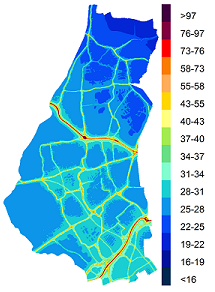
\includegraphics{images/no2_2020_raster.png}
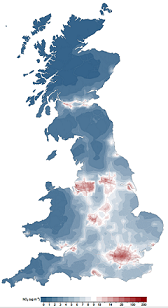
\includegraphics{images/cmaq_uk_v2.png}
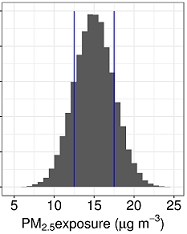
\includegraphics{images/theoretical_lhem_pm25.png}

\begin{itemize}
\tightlist
\item
  Now at Guy Carpenter (Model development, Re-insurance)
\end{itemize}

\hypertarget{why-measure-air-on-the-tube}{%
\subsection{Why measure air on the
tube}\label{why-measure-air-on-the-tube}}

\begin{itemize}
\item
  Exposure to particles on subway systems \textgreater{} important
\item
  Seaton et al 2005, but \ldots{}

  \begin{itemize}
  \tightlist
  \item
    Tox. mechanisms
  \item
    Susceptible populations
  \item
    Analytical techniques
  \end{itemize}
\end{itemize}

\hypertarget{aims}{%
\section{Aims}\label{aims}}

\hypertarget{what-we-tried-to-do}{%
\subsection{What we tried to do}\label{what-we-tried-to-do}}

\begin{itemize}
\tightlist
\item
  Measure variations in PM2.5 between lines and stations
\item
  Characterise the chemical composition
\item
  Calculate calibration factors for optical instruments
\item
  Provide a spatially resolved dataset for future analysis
\end{itemize}

\hypertarget{method}{%
\section{Method}\label{method}}

\hypertarget{mobile-measurement-campaign}{%
\subsection{Mobile Measurement
campaign}\label{mobile-measurement-campaign}}

\begin{itemize}
\tightlist
\item
  TSI AM510 SidePak (PM2.5)
\item
  Philips Aerasense (numbers and size of particles)
\item
  31 hours
\item
  All lines
\item
  89\% of stations (NE Central, SW Piccadilly)
\end{itemize}

\hypertarget{geo-tagging-data}{%
\subsection{Geo-tagging data}\label{geo-tagging-data}}

\begin{itemize}
\tightlist
\item
  Need to link air quality measurements to locations
\item
  No GPS signal on large sections of the network
\item
  Considered using timetables / interpolating between known locations
\item
  Ended up using a notepad
\end{itemize}

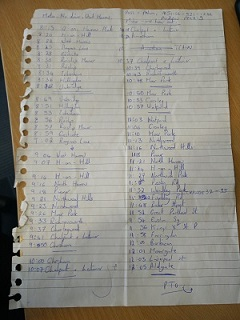
\includegraphics{images/metropolitan_line_1.jpg}
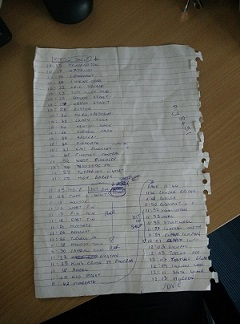
\includegraphics{images/northern_line_2.jpg}
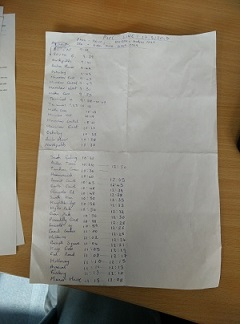
\includegraphics{images/Piccadilly_Line_1.jpg}

\hypertarget{characterisation-calibration}{%
\subsection{Characterisation \&
Calibration}\label{characterisation-calibration}}

\begin{itemize}
\tightlist
\item
  Tricky installation at Hampstead
\item
  Particles collected on filters over 5 days measuring composition \&
  amount
\item
  High time resolution equipment installed

  \begin{itemize}
  \tightlist
  \item
    Aethalometer / TSI Dustrak / 2 TSI Sidepaks / Micro-aethalometer
  \end{itemize}
\end{itemize}

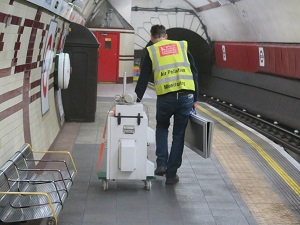
\includegraphics{images/hampstead_equipment.jpg}
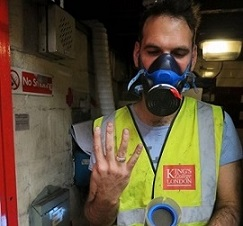
\includegraphics{images/max_characterisation.jpg}

\hypertarget{passenger-weighted-stations}{%
\subsection{Passenger-weighted
stations}\label{passenger-weighted-stations}}

\begin{itemize}
\tightlist
\item
  2015 tap in/tap out, Underground performance report
\item
  Annual in/out for each station
\item
  Mean PM2.5 measured at each station
\item
  Passenger rank * air quality rank = passenger-weighted ranking
\end{itemize}

\hypertarget{spatial-representation-of-the-tube}{%
\subsection{Spatial representation of the
tube}\label{spatial-representation-of-the-tube}}

\hypertarget{results}{%
\section{Results}\label{results}}

\hypertarget{calibration-factors}{%
\subsection{Calibration factors}\label{calibration-factors}}

\begin{itemize}
\tightlist
\item
  Linear model to calculate correction factors for mobile monitoring
  equipment
\item
  Mobile monitoring equipment co-located in tube station v. outdoor
\end{itemize}

\hypertarget{the-victoria-line}{%
\subsection{The Victoria Line}\label{the-victoria-line}}

\hypertarget{line-averages}{%
\subsection{Line averages}\label{line-averages}}

\hypertarget{station-depth-1}{%
\subsection{Station depth 1}\label{station-depth-1}}

\hypertarget{station-depth-2}{%
\subsection{Station depth 2}\label{station-depth-2}}

\hypertarget{depth-on-the-central-line}{%
\subsection{Depth on the Central Line}\label{depth-on-the-central-line}}

\hypertarget{pm2.5-map}{%
\subsection{PM2.5 Map}\label{pm2.5-map}}

\hypertarget{pm2.5-online-map}{%
\subsection{PM2.5 online map}\label{pm2.5-online-map}}

\href{http://www.erg.kcl.ac.uk/research/home/projects/TubeMapPM25.html}{Online}

\hypertarget{passenger-weighted-stations-1}{%
\subsection{Passenger-weighted
stations}\label{passenger-weighted-stations-1}}

\hypertarget{origin-destination-matrix}{%
\subsection{Origin-Destination matrix}\label{origin-destination-matrix}}

\hypertarget{characterisation}{%
\subsection{Characterisation}\label{characterisation}}

\hypertarget{conclusions}{%
\section{Conclusions}\label{conclusions}}

\hypertarget{conclusions-1}{%
\subsection{Conclusions}\label{conclusions-1}}

\begin{itemize}
\tightlist
\item
  Particles tend to be larger in diameter than those at background or
  roadside environments
\item
  More particles
\item
  PM2.5 varied between lines \& locations

  \begin{itemize}
  \tightlist
  \item
    lowest Hammersmith \& City (Mean 25 µg/m3), similar to roadside
  \item
    highest Victoria (381 µg/m3), 15 x higher than roadside
  \end{itemize}
\end{itemize}

\hypertarget{conclusions-2}{%
\subsection{Conclusions 2}\label{conclusions-2}}

\begin{itemize}
\tightlist
\item
  General relationship between `depth' and air quality
\item
  Oxford Circus, Waterloo, London Bridge, Victoria and Vauxhall at top
  of passenger-exposure ranking
\item
  79\% of PM2.5 characterised

  \begin{itemize}
  \tightlist
  \item
    47\% iron oxide, 7\% elemental carbon, 11\% organic carbon, 14\%
    metallic and mineral oxides
  \end{itemize}
\item
  Previous studies using light-scattering may under-report PM
\end{itemize}

\hypertarget{what-next}{%
\section{What next}\label{what-next}}

\hypertarget{what-was-planned}
\item
  \sout{More measurements accross the network to improve understanding}

  \begin{itemize}
  \tightlist
  \item
    \sout{train frequency}
  \item
    \sout{passenger numbers}
  \item
    \sout{time of year}
  \end{itemize}
\item
  \sout{Interventions?}
\item
  \sout{Develop inclusion in exposure modelling}
\end{itemize}

\hypertarget{what-happened}{%
\subsection{What happened}\label{what-happened}}

\includegraphics[width=0.3\textwidth,height=\textheight]{images/lola_swing.gif}
\includegraphics[width=0.3\textwidth,height=\textheight]{images/lola_swing.gif}

\hypertarget{the-end}{%
\section{The end}\label{the-end}}

\hypertarget{publication-contact-data}{%
\subsection{Publication, Contact \&
Data}\label{publication-contact-data}}

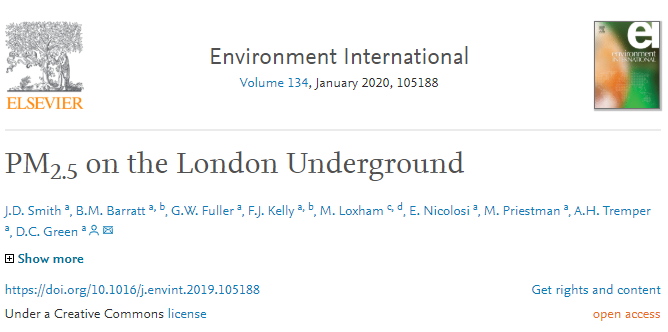
\includegraphics{images/tube_paper.png} CSV of data available at:
\url{https://data.mendeley.com/datasets/tv56txbpcw/1}

\includegraphics{images/email_logo.jpg}
\href{mailto:james.d.smith@gmail.com}{\nolinkurl{james.d.smith@gmail.com}}
\includegraphics{images/email_logo.jpg}
\href{mailto:james.d.smith@guycarp.com}{\nolinkurl{james.d.smith@guycarp.com}}

\includegraphics{images/twitter_logo.png}
\href{http://twitter.com/therealjimshady}{TheRealJimShady}


\end{document}
